%==================================
% (c) Jan Tulak, 2017
%%%%%%%%%%%%%%%%%%%%%%%%%%%%%%%%%%%%%%%%%%%%%%%%%%%%%%%%%%%%%%%%%%%%%%%%%%%%%

\chapter{Results}\label{chap:results}
%----------------------------------------------------------------------

In this chapter, the results of every tool are compared and analysed. If not
stated otherwise, the number of issues is for mkfs-specific files, i.e., for
files in {\tt mkfs/} directory. Every tool has its own section in which its
performance is analysed across of multiple revisions of mkfs in detail.

\Cref{tab:results:overview} offers an overview of how many issues did every
tool find on various revisions. These revisions are stored in the project's git
repository and they are identified by their hash, so this table also shows
which revision follows which.  Selected revisions (annotated with {\em total
issues}) shows the number of outstanding issues on this specific point of
development.

For the remaining revisions, the table shows new/fixed issues: $+x$ denotes the
number of new issues found, $-x$ denotes the number of issues fixed between this
and the previously tested revision. For example, revision {\tt a887c950} has a
value $+1$/$-3$ for Coverity. That means that, according to Coverity, one new
issue appeared in this revision, while 3 others were fixed. A zero, in this
case, means no change.  A --- dash means that the tool was not used in this
specific revision.  The numbers of issues were gained with every tool set up to
the strictest analysis.

\begin{table}[h]
\begin{tabular}{|r||r|r|r|r|r|r|}
\hline
Commit & CppCheck & Codacy & CPAChecker & Coverity & GCC & Clang \\
\hline
\hline
\multicolumn{7}{|c|}{Total issues}\\
\hline
(tag: v4.11.0-rc1) {\tt 07a3e793} & $1$ & $3$ & & $119$ & $30$ & $34$ \\
\hline
(tag: v4.7.0) {\tt d7e1f5f1} & $1$ & $4$ & & $119$ & $30$ & $28$ \\
\hline
\hline
\multicolumn{7}{|c|}{Changes}\\
\hline
{\em [Last of my set]} {\tt 2aca16d6} & 0 & 0 & & 0 & 0 & 0 \\
\hline
{\tt aa3034d4} & 0 & 0 & & $+2$/$-2$ & 0 & 0 \\
\hline
{\tt 6de2e6c0} & 0 & 0 & & $+5$ & 0 & 0 \\
\hline
{\tt ddc3b2da} & 0 & 0 & & 0 & 0 & 0\\
\hline
{\tt 06ac92fd} & 0 & 0 & & $+12$/$-3$ & $+1$ & $+1$\\
\hline
{\tt 27ae3a59} & 0 & 0 & & $+1$ & 0 & 0 \\
\hline
{\tt 3ec1956a} & 0 & 0 & & $+1$/$-3$ & 0 & 0 \\
\hline
{\tt 6c855628} & 0 & 0 & & $+2$/$-2$ & $-2$ & $-2$ \\
\hline
{\tt 627e74fd} & $-3$ & $-2$ & & 0 & $+2$ & $+2$ \\
\hline
{\tt 9090e187} & 0 & 0 & & $+2$ & 0 & 0 \\
\hline
{\tt 1974d3f1} & 0 & 0 & & 0 & $-1$ & 0 \\
\hline
{\tt 56e4d368} & 0 & 0 & & $-3$ & 0 & 0 \\
\hline
{\tt a9dad670} & 0 & 0 & & $+4$ & $-54$ & $-54$ \\
\hline
{\tt 147e0f31} & 0 & 0 & & $+3$ & 0 & 0 \\
\hline
{\tt c81c8460} & 0 & 0 & & 0 & $-50$ & $-50$ \\
\hline
{\tt a887c950} & 0 & 0 & & $+1$/$-3$ & $+13$ & $+12$ \\
\hline
{\tt 5f1a2100} & 0 & 0 & & 0 & 0 & 0 \\
\hline
{\tt ff21c709} & 0 & 0 & & 0 & $+1$ & $+1$ \\
\hline
{\em [First of my set]} {\tt 4a32b9e9} & $-1$ & $-1$ & & 0 & 0 & 0 \\
\hline
\hline
\multicolumn{7}{|c|}{Total issues} \\
\hline
{\em [Before my set]} {\tt 6aa32b47} & $5$ & $6$ & & $111$ & $121$ & $117$ \\
\hline
(4.6.0) {\tt 09033e35} & $5$ & $6$ & & $111$ & $121$ & $117$ \\
\hline
\end{tabular}
\caption{An overview of issues found by the tested tools on specific revisions
	in mkfs-only files.}
\label{tab:results:overview}
\end{table}

It is apparent from the table, even on the first glance, that the performance
of the tools varies widely. Not only in absolute numbers of reported issues (of
which some are false positives), but also in detecting specific issues. For
example, revision {\tt a9dad670} fixed 54 issues according to GCC, but
according to Coverity, it caused 4 new and did not fix anything.

Bellow, we have both a simple statistical analysis of what each
tool found and a more detailed look at some specific issues and revisions,
especially where the tools have seriously different results.



%======================================================================
\section{CppCheck}\label{chap:results:cppcheck}
%----------------------------------------------------------------------
CppCheck (and Codacy, which is using it) found fewer issues than other
tools. When the kind of issues found is analysed, it becomes apparent that
this tool is greatly limited. Still, this tool is the easiest to use and it is
open source, which can make it a useful entry point for projects that do not
use any other form of analysis.

The only two revisions we mention here are v4.6.0 and 4.7.0, before and after
our patches. The differences between other revisions are negligible.

In version 4.6.0, 5 issues were found in mkfs-specific
files, and 460 issues in whole xfsprogs. From these, 100 issues were not
stylistic.

The issues found in mkfs are:
\begin{enumerate}
	\item {\tt mkfs/xfs\_mkfs.c:1067}: Checking if unsigned variable
		'blocksize' is less than zero.
	\item {\tt mkfs/xfs\_mkfs.c:1698}: Checking if unsigned variable
		'sectorsize' is less than zero.
	\item {\tt mkfs/xfs\_mkfs.c:1225}: Checking if unsigned variable
		'sectorsize' is less than zero.
	\item {\tt mkfs/xfs\_mkfs.c:2487}: Condition '0' is always false
	\item {\tt mkfs/xfs\_mkfs.c:2733}: The scope of the variable 'bucket'
		can be reduced.
\end{enumerate}

All these issues were present for multiple years. Precise dating is
difficult, however, because e.g. issue 1 is blamed to a commit 16 years
old. But at that time, the variable was signed. Thus, the issue appeared
some time later, when the specific variable was turned to unsigned, but not
every use was fully converted.

Neither of these issues is of any seriousness. Every found check of an
unsigned variable to being lower than zero is, in fact, a less-or-equal
check. \Cref{lst:results:sectorsize} shows the specific code for both cases
of offending sectorsize. Thus, {\tt unsigned\_variable <= 0} may be
misleading, but functionally is equivalent to {\tt unsigned\_variable ==
0}.  And the condition '0' being always false is a value intentionally
passed to a macro.

Other tools do not report this case of unsigned variable comparison,
likely because the lower-than symbol, in this case, does not have any effect.

\begin{lstlisting}[frame=none, basicstyle=\footnotesize\ttfamily,
language=C, numbers=none, numberstyle=\tiny\color{black},caption=
{Condition in which unsigned sectorsize is tested to be less than zero.},
label={lst:results:sectorsize}]
if (sectorsize <= 0 || !ispow2(sectorsize))
	// do something
\end{lstlisting}

The patches we wrote removed most of the offending code, so only 1 issue was
found in mkfs-specific files in version 4.7.0. In that version in the whole
xfsprogs, 440 issues were found, from which 100 issues were not style issues.

The issue found in mkfs  is:\\
{\tt mkfs/xfs\_mkfs.c:2918}: The scope of the variable 'bucket' can be reduced.

When compared with Codacy, CppCheck reports one issue twice: Checking if an
unsigned variable is less than zero. This happens in two places, but Codacy
ignores the second occurrence. On the other side, CppCheck did not find any
issue in {\tt mkfs/proto.c} file, where Codacy did.

These differences might be caused by a different configuration of CppCheck,
because we used the default configuration, but do not know what changes
Codacy did.

Despite this, the results of those two tools are very similar when compared
to others, so we use only CppCheck in further comparison with other tools.
CppCheck is selected because we have greater control over it, unlike cloud
service Codacy, and on this sample produced no false positives, although the
usfullness of some reports is arguable.

The low number of issues found can be attributed to the detailed review of all
patches submitted to the project. If most issues are usually spotted during the
development in the patches and fixed before they are merged into the code, it
leaves space for only more complex and not so obvious issues, which CppCheck
analysis is not capable of finding and a stronger tool is necessary.

%======================================================================
\section{Codacy}\label{chap:results:codacy}
%----------------------------------------------------------------------
Codacy shows only per-commit and total issues for a branch. That is, a
developer can view whether a specific commit fixed or caused an issue, and
can see what are the issues for the top of the repository, but checking the
complete state at a particular point in the history requires creating a new
branch, which is uncomfortable, but manageable for a private\footnote{In
the sense of being the only user, not in terms of visibility.} repository.
In a repository with many contributors, it can be confusing.

Codacy provides some rating on the project's page~\cite{codacyXfsprogs},
which considers xfsprogs as a quality project (A-grade), but the weight of
this rating is unclear and rather informal. Also, it is not clear without
checking every issue, what metrics Codacy uses to assess the type, whether
it is style, error or security issue.

In mkfs-specific files in version 4.6.0, 6 issues were found. Whole
xfsprogs had 839 issues, from which 809 were code style issue and 30 were
potential errors.

Codacy found most of the same issues as CppCheck with few exceptions. It
reported these two issues:
\begin{enumerate}
	\item {\tt mkfs/proto.c:49}: The function 'setup\_proto' is never used.
	\item {\tt mkfs/proto.c:601}: The function 'parse\_proto' is never used.
\end{enumerate}

However, these functions are used in {\tt mkfs/xfs\_mkfs.c} file, thus they are
false positives. Also, CppCheck found two places on which {\tt sectorize} is
checked to be less than zero, but Codacy reports it only once. Curiously, the
same issue appears on two places not far away, and in both cases, it is in this
exact condition as can be seen in \Cref{lst:results:sectorsize} in
\Cref{chap:results:cppcheck}, just inside of different blocks, but still in the
same function and path to both places is possible. Why Codacy does report only
one of those issues is unclear.


In version 4.7.0 in mkfs-specific files, 4 issues were found. Whole
xfsprogs had 749 issues, from which 719 were code style issue and 30 were
potential errors.

The four issues found in this version are similar to what can be seen for the 4.6.0:
\begin{enumerate}
	\item {\tt mkfs/xfs\_mkfs.c:2918}: The scope of the variable {\tt
		bucket} can be reduced.
	\item {\tt mkfs/maxtrres.c:31}: The function {\tt max\_trans\_res}
		is never used.
	\item {\tt mkfs/proto.c:49}: The function {\tt setup\_proto} is
		never used.
	\item {\tt mkfs/proto.c:601}: The function {\tt parse\_proto} is
		never used.
\end{enumerate}

Also in this case, the supposedly unused function {\tt max\_trans\_res} is
in fact used in another file.

In total, Codacy results are similar to CppCheck itself, but with more of false
positives. The only advantage it offers is automated integration with GitHub.
With a correct set-up, it can ensure that every push into the repository is
tested.

%======================================================================
\section{GCC and Clang}\label{chap:results:gcc}
%----------------------------------------------------------------------

Despite being developed independently, GCC and Clang are very similar in what
they found, with GCC finding a few more issues. In this section, we describe
some of the notable differences between those two tools and compare them to
others where it is reasonable.

% ------------------------------------------------
\subsection{Version 4.6.0}\label{chap:results:gcc:4.6}

\Cref{tab:results:gcc:4.6} compares GCC and Clang in this revision, and we
specifically look at the differences between these two tools and Codacy.
Other issues are not listed here due to their amount, but the reader can find
them on an attached optical disc, or replicate them using the tools attached to
this work.

\begin{table}[h]
\begin{tabular}{|l||r|r||r|}
\hline
Tool & {\tt mkfs/xfs\_mkfs.c} & {\tt mkfs/proto.c} & Whole xfsprogs \\
\hline
GCC & 121 & 2 & 2013 \\
\hline
Clang & 113 & 4 & 2597 \\
\hline
\end{tabular}
\caption{Comparison of the number of issues reported by GCC and Clang in version
4.6.0.}
\label{tab:results:gcc:4.6}
\end{table}

As is shown in \Cref{chap:results:codacy}, Codacy found two issues in the {\tt
proto.c} file too. Curiously, Codacy found two unused functions, while GCC
found these issues:
\begin{enumerate}
	\item {\tt mkfs/proto.c:270}: comparison between signed and unsigned
		integer expressions
	\item {\tt mkfs/proto.c:332}: unused parameter 'mp'
\end{enumerate}

These issues are not in the two functions found by Codacy. However, they are
inside of functions called from the ones marked as unused by Codacy. It is
possible that they were not reported because of this, but given that the
mentioned Codacy issues are false positives and that Codacy did not found many
other issues, it is likely that Codacy simply did not notice them, while GCC
did.

In addition to the two issues found by GCC in {\tt mkfs/proto.c}, Clang
found two other issues (both of the same kind):
\begin{enumerate}
	\item {\tt mkfs/proto.c:130}: missing field 'tr\_logcount' initializer
	\item {\tt mkfs/proto.c:631}: missing field 'tr\_logcount' initializer
\end{enumerate}

These two new issues, complaining about a missing field, are probably false
positives because, on these lines, a structure with all members zeroed is
created, as can be seen in \Cref{lst:results:zeroedStruct}.

\begin{lstlisting}[frame=none, basicstyle=\footnotesize\ttfamily,
language=C, numbers=none, numberstyle=\tiny\color{black},caption=
{One of the two lines on which Clang reports a missing field in structure
initialization.},
label={lst:results:zeroedStruct}]
struct xfs_trans_res    tres = {0};
\end{lstlisting}

The difference between GCC and Clang in {\tt mkfs\_xfs.c} file is 8 issues in
absolute numbers, and the real difference is not much bigger; GCC reports more
cases of a comparison between signed and unsigned integer than Clang does.
Clang, on the other hand, reports few cases of this issue:

{\tt mkfs/xfs\_mkfs.c:2906} cast from 'char *' to 'xfs\_alloc\_rec\_t *' (aka
'struct xfs\_alloc\_re    c *') increases required alignment from 1 to 4

Other than that, they report the same issues.

% ------------------------------------------------
\subsection{Revision a887c950}\label{chap:results:gcc:a887c950}
GCC detected 13 new issues in {\tt mkfs/xfs\_mkfs.c}. These 13 issues are only of two
kinds:
\begin{enumerate}
	\item {\tt mkfs/xfs\_mkfs.c:1487}: comparison is always false due
		to limited range of data type
	\item {\tt mkfs/xfs\_mkfs.c} {\em multiple occurencies}: passing
		argument 2 of 'illegal' discards 'const' qualifier from
		pointer target type
\end{enumerate}

Clang detected all the 12 occurrences the second issue but missed the first,
comparison issue. The offending line for the missed issue is shown in
\Cref{lst:results:logagnoComparison}. A closer look on this line reveals that
there is an explicit type casting. The new type is a signed integer. However,
the variable {\tt logagno} is declared with type {\tt xfs\_agnumber\_t} and
this type is declared as an alias to {\tt \_\_uint32\_t} in file {\tt
libxfs/xfs\_types.h}.

According to the standard of C language, the type casting has a precedence over
comparison~\cite[A.2.1]{ISO9899}, so Clang, when evaluating this line, sees
an integer. That is technically correct, but in a wider context, it is also
clear that the possible values are still limited by the original type, and
so this comparison will be always false.  Which is what GCC noticed and
also correctly reported. No other tool reported this issue.

\TODO{Will CPA report this once it is working?}

\begin{lstlisting}[frame=none, basicstyle=\footnotesize\ttfamily,
language=C, numbers=none, numberstyle=\tiny\color{black},caption=
{Line on which GCC found the comparison issue.},
label={lst:results:logagnoComparison}]
if ((__int64_t)logagno < 0)
	// do something
\end{lstlisting}

The other issues are similar to what Clang found but appears to suffer the
instability in parsing mentioned in \Cref{chap:techniques:processing}.
All these issues are caused by passing a constant string to a
function which does not has the {\tt const} keyword for an argument: {\tt
illegal(value, "b log");}. The file {\tt xfs\_mkfs.c} contains 44 such
calls, but only some of them were added in this revision. Thus, we correctly
detected these issues, but some of the line numbers we see had this issue
before. If we would want to see exactly which lines were added, the easiest way
is to look to look at changes in this specific commit.


% ------------------------------------------------
\subsection{Version 4.7.0}\label{chap:results:gcc:4.7}

Clang found 3 more issues in this revision than GCC did in file {\tt
mkfs/proto.c}, as is shown in the comparison in \Cref{tab:results:gcc:4.7}. Two
of them already appeared in the description of revision 4.6 in
\Cref{chap:results:gcc:4.6} and were not fixed, the third issue is of the same
kind and was introduced by some other patch other than which are part of this
work.

\begin{table}[h]
\begin{tabular}{|l||r|r||r|}
\hline
Tool & {\tt mkfs/xfs\_mkfs.c} & {\tt mkfs/proto.c} & Whole xfsprogs \\
\hline
GCC & 28 & 2 & 2013 \\
\hline
Clang & 23 & 5 & 2511 \\
\hline
\end{tabular}
\caption{Comparison of the number of issues reported by GCC and Clang in version
4.7.0.}
\label{tab:results:gcc:4.7}
\end{table}

Almost all issues found in {\tt mkfs/xfs\_mkfs.c} are about a comparison, with
only two exceptions:
\begin{enumerate}
	\item {\tt mkfs/xfs\_mkfs.c:728}: unused parameter 'lsectsz'
	\item {\tt mkfs/xfs\_mkfs.c:1896}: passing argument 2 of 'unknown'
		discards 'const' qualifier from pointer target type
\end{enumerate}


Most issues in Clang are also about a comparison, with multiple versions of
wording, because where GCC uses only one universal message, Clang uses a
template into which it substitutes specific types. This makes the analysis of
the results more challenging but does not have any effect on the results.
In this revision, Clang does not report any new kind of issues against version
4.6.0.

%======================================================================
\section{Coverity}\label{chap:results:coverity}
%----------------------------------------------------------------------

Coverity, when it is run manually in the docker container, found a comparable
number of issues as GCC and Clang in mkfs-specific files. On the other hand,
the online version did not found any issues in mkfs on a recent (4.11)
version~\cite{CoverityXfsprogs}, compared to 111 found on a manual run with the
highest level of aggressiveness. What effect the aggressiveness level has can
be seen in \Cref{tab:results:coverity:levels}. The numbers in this table are
for mkfs-specific files. The tested revision is {\tt 07a3e793} (v4.11.0-rc1).
From the results, it is probable that the service is using configuration similar
to the low aggressiveness.  Especially when numbers for the whole xfsprogs are
compared.


\begin{table}[h]
\begin{tabular}{|l||r|r|r|r|r|}
\hline
& online & low & medium & high & custom \\
\hline
Issues reported & 0 & 0 & 36 & 97 & 111 \\
\hline
\end{tabular}
\caption{Comparison of issues found by Coverity online service and Coverity run
locally with different levels of aggressiveness.}
\label{tab:results:coverity:levels}
\end{table}

In most of this section, we focus on results gained from the custom (highest)
level. The online service is briefly described and some interesting statistics
comparing xfsprogs with other open-source projects (in an aggregated manner)
are provided only in \Cref{chap:results:coverity:online}.

The reasons for selecting the custom level aggressiveness as the level on which
our analysis focusses is that for other tools we used the strictest settings
available, thus, analysing relaxed approach on any other level is not
comparable to other tools.

Unlike CppCheck or the compilers, Coverity can also show examples of the data
flow for which a defect can appear.  E.g. tracking multiple conditions and
noting if true or false branch was taken. This is especially useful when the
case is not clear and the path includes a longer chain of conditions over a
larger part of the code. Both the online service and the locally-run
application provides this information. However, it is not particularly useful
in our comparison of what issues were found.

% ------------------------------------------------
\subsection{Online Service}\label{chap:results:coverity:online}

The online service available at
\url{https://scan.coverity.com/projects/xfsprogs} provides various statistics
in addition to reported issues. The online service found no issues in mkfs. In
whole xfsprogs, it reported 71 issues, which is similar to what the manual
execution on the low level found (77 issues). The service also provides a view on
specific categories, as can be seen in \Cref{fig:results:coverity:defects}

\begin{figure}
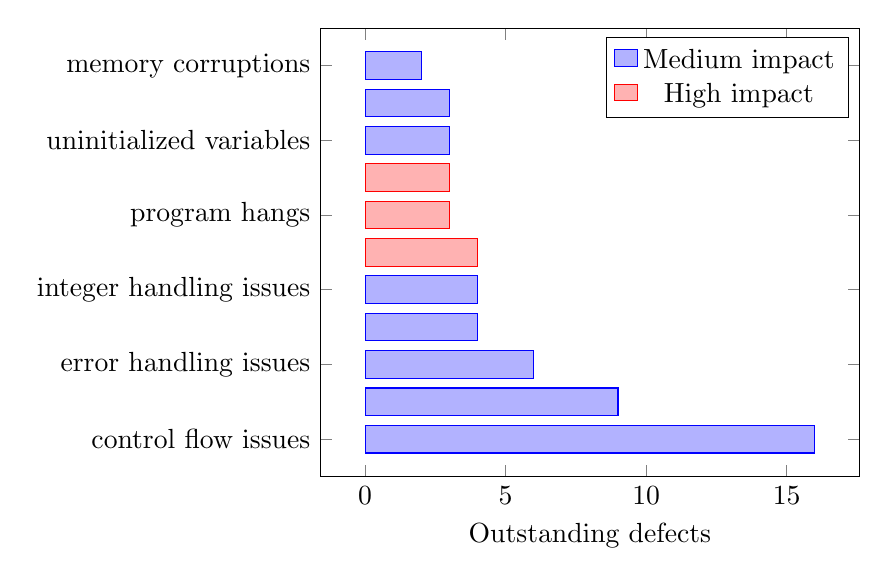
\begin{tikzpicture}
	\begin{axis}[
		xlabel={Outstanding defects},
		yticklabels={null pointer dereference,
			control flow issues,
			error handling issues,
			integer handling issues,
			program hangs,
			uninitialized variables,
			memory corruptions,
			memory illegal access,
			API usage errors,
			insecure data handling,
			concurent data access},
		y tick label style={rotate=0,anchor=east},
		xbar stacked,
	]
	\addplot
	coordinates {
		(16,0)(9,1)(6,2)(4,3)(4,4)(0,5)(0,6)(0,7)(3,8)(3,9)(2,10)
	};
	\addlegendentry{Medium impact}
	\addplot
	coordinates {
		(0,0)(0,1)(0,2)(0,3)(0,4)(4,5)(3,6)(3,7)(0,8)(0,9)(0,10)
	};
	\addlegendentry{High impact}
	\end{axis}
\end{tikzpicture}
\caption{Outstanding deffects per category.}
\label{fig:results:coverity:defects}
\end{figure}

This service is used since 2013 and since xfsprogs was first analysed, a total
number of 273 issues was found. Of these, 176 was fixed and 26 dismissed as
intentional or false positives. The average defect density according to this
analysis is currently 0.52 issues per 1,000 lines, with 135,302 lines analysed.

When xfsprogs was analysed for the first time by this service, 139 issues were
found, but many were fixed shortly afterwards and the number of outstanding
defects is not changing much, averaging between 60 and 70 issues at any
specific revision. When compared with other open-source projects of similar
size\footnote{100,000 to 400,000 lines of code.} analysed by this service,
xfsprogs oscillates around the average value, which is 0.5.

It is also useful to note that the defects are not distributed equally in the
whole xfsprogs. When we look at the defects rate per component, seen in
\Cref{tab:results:coverity:components}, we can see that the tools used by
developers for e.g. debugging, or by advanced users ({\tt xfs\_copy}, {\tt
xfs\_logprint}) have a higher rate than the tools intended for a general use,
like {\tt mkfs}. The high rate in {\tt libxcmd} and {\tt libhandle} is caused
by the small size of these two components. Both has only a single issue, but as
{\tt libhandle} has under 500 lines, the average per 1000 lines makes it look
worse.


\begin{table}[h]
\begin{tabular}{|l||r|r|r|r|r|r|r|}
\hline
 & libxfs & libxlog & xfs\_repair & xfs\_db & xfs\_copy & xfs\_fsr & xfs\_io  \\
\hline
Lines of code & 43,770 & 1,165 & 22,620 & 18,508 & 1,043 & 1,354 & 6,970  \\
\hline
Defect density & 0.80 & 0.86 & 0.44 & 0.49 & 2.88 & 0.74 & 0.00 \\
\hline
\hline
 & xfs\_logprint & xfs\_quota & mkfs\_xfs & xfs\_growfs & libhandle & libxcmd & other \\
\hline
Lines of code & 2,616 & 4,037 & 3,540 & 408 & 493 & 1,338 & 27,539 \\
\hline
Defect density & 1.15 & 0.50 & 0.00 & 0.00 & 2.03 & 1.38 & 0.15 \\
\hline
\end{tabular}
\caption{Defect density per component as reported by Coverity online service.}
\label{tab:results:coverity:components}
\end{table}

% ------------------------------------------------
\subsection{Local analysis}\label{chap:results:coverity:local}

This section analyses the results from the local execution of Coverity on the
highest level of aggressiveness.

In mkfs-specific files in version 4.6.0, 111 issues were found, while whole xfsprogs
had 3309 issues. From the issues reported for mkfs, 60 is a complaint about
dereferencing a pointer that might be null in {\tt printf} or {\tt fprintf}
call.

An example of a line with such a warning is in
\Cref{lst:results:dereferencePrintf}. The issue lies with
Gettext\footnote{Gettext is a tool/library for translation of programs. It
generates a list of marked string from a program. These string can be
translated and packaged with the compiled program. When the program is run,
Gettext selects the correct language based on system configuration.}. The {\tt
\_}
macro is translated as a {\tt dcgettext} call and it is the result of this
function that Coverity can't verify. And because there is no check of the
return value for null before it is passed to {\tt printf}, Coverity makes an
aggressive assumption and raise a warning.

\begin{lstlisting}[frame=none, basicstyle=\footnotesize\ttfamily,
language=C, numbers=none, numberstyle=\tiny\color{black},caption=
{{\tt xfs\_mkfs.c:1713}: Line which is reportedly dereferencing a potentially
null pointer with Gettext},
label={lst:results:dereferencePrintf}]
printf(_("%s version %s\n"), progname, VERSION);
\end{lstlisting}

These issues can be probably considered false positives, or at least
intentional. A brief search in Gettext implementation suggests that if Gettext
cannot allocate memory for a translated string, it simply returns the original
one. For example, see file {\tt /gettext-runtime/intl/dcigettext.c}, line 391
in Gettext source code~\cite{GettextGit}.

Only 10 of the dereferencing issues are related to something else
than {\tt dcgettext} and might be useful. An example of such issue is
\Cref{lst:results:dereferenceBuf}.  In this case, memory is allocated with a
{\tt malloc} call. The returned value is not tested, so it is possible that
null is passed to the {\tt read} call.

\begin{lstlisting}[frame=none, basicstyle=\footnotesize\ttfamily,
language=C, numbers=none, numberstyle=\tiny\color{black},caption=
{{\tt proto.c:66}: Line which is reportedly dereferencing a potentially null
pointer - no malloc check.},
label={lst:results:dereferenceBuf}]
buf = malloc(size + 1);
if (read(fd, buf, size) < size) {
        // do something...
\end{lstlisting}

These two issues also illustrate the difference between the aggressiveness
level. The Gettext-related issue is reported only on high or custom level, but
the malloc issue is reported also on medium level.

When compared to GCC or Clang, Coverity finds different issues than the other
tools. While GCC reports a lot of comparison between signed and unsigned
integers or discarding {\tt const} qualifier, Coverity finds a lot of potential
null pointer dereferences and numeric types overflows when 32bit and 64bit
arithmetics are mixed.

%======================================================================
\section{CPAChecker}\label{chap:results:cpachecker}
%----------------------------------------------------------------------

%======================================================================
\section{Summary}\label{chap:results:summary}
%----------------------------------------------------------------------

As we have seen, the results of the tools vary widely, both in types of issues
the tools report and in their amount.  The mediocre results of CppCheck and
Codacy can be probably attributed to the fact that we tested it on a production
code which already passed a certain quality assurance and thus, the kinds of
issues these tools are best capable of finding were already fixed.

Coverity and both compilers were capable of finding less obvious defects, but
the price for a too high sensitivity was a lot of reported issues with only a
minimal, if any, effect, like the comparisons between signed and unsigned
integers from GCC.

In any case, this work shows that on a relatively error-free code, there is
only a minimum of defects that would be reported by multiple tools. This makes
it apparent that it is useful to use as many diverse methods in the analysis as
possible.

The most helpful tool from the tested ones was Coverity, not least because of
its ability to show the flow of the program in which the defect can appear.
However, the free analysis for open source projects is limited to more obvious
defects and for non-open source projects, or for a detailed analysis, it
requires a paid license.

This analysis was done after the first patches were written and merged, but
found minor issues only, which speaks well for the quality of mkfs, at least in
terms of correctness with respect to the language standard. Whether the code is
well structured or not, or if it does what is expected from it on a higher
level, is not possible to assess with these tools.

